\chapter{Physics II}
This compendium is based on the course notes of MIT 8.02 2004 \url{https://web.mit.edu/8.02t/www/802TEAL3D/visualizations/coursenotes/index.htm} and the lectures of MIT 8.02 by Professor Walter Lewin in 2002. The video lectures can be viewed on YouTube from Lectures by ``Walter Lewin. They will make you \ensuremath\varheartsuit~Physics.'' with the playlist name ``8.02x - MIT Physics II: Electricity and Magnetism''
All credits go to Dr. Sen-ben Liao, Dr. Peter Dourmashkin, and Professor John W. Belcher at MIT for the lecture notes and Professor Walter Lewin for the inspiring lectures. I can not guarantee the accuracy of this compendium and that it is a correct interpretation of the material and explanation provided by the lecture notes and lectures. Thus, for accurate information refer to the material that this compendium is based on. If a mistake is in the compendium it is most likely my fault and not the fault of the material in which this compendium is based on.


%\section{Introduction}
\section{Electric Charges}
%\section{Electric Charges and Forces and Coulomb's Law - Polarization}
An atom comprises positively charged protons, neutrally charged neutrons, and negatively charged electron.
An atom or molecule can have a neutral, positive or negative electric charge. A negatively charged atom or molecule is called a \textit{negative ion}, meaning to a surplus of electrons compared to protons.
A positively charged atom or molecule is called a \textit{positive ion}.
The nucleus, the protons and neutrons or the atom, is significantly larger than an electron, a proton with a size of $10^{-15}\SI{}{\meter}$ is roughly 1000 times larger than an electron with a size of $10^{-18}\SI{}{\meter}$.
For a hydrogen atom the lower energy state has the most probable distance, using Bohr Radius, of approximately $10^{-11}\SI{}{\meter}$ from the nucleus, which is 10000 times further than the size of the hydrogens' proton.

An intuitive way of thinking why same changed ions repel each other and why opposite charged ions attracted each other is to think about a room where we have loud and talkative people who want someone to listen to them, i.e., negative ions, and quiet, shy listeners, positive ions. When a loud and talkative person is approached by another loud and talkative person they talk over each other and neither gets want they want and find it physically uncomfortable to be near each other, they naturally repel each other. Likewise, if two quite people talk to each other they find it awkward and physically uncomfortable to be close each other. However, if there are a quite, shy listener and a loud talkative person they have found there mach.

Conductors allows electrons to flow ``freely'', there is always some resistance. Continuing with our metaphor we can think of it as a channel where the voice of the loud and talkative person can travel far and reach the quite, shy listener. And non-conductors are like a wall where the voice does not travel through.

\section{Polarization}

If we have a positive charge object like we see with the rod in Figure~\ref{fig:charged-rod} placed next to a conductive object like we see with the cloud shaped object next to the rod, the conductive object will have a negative and a positive charged side. Only $10^{13}$ of electrons that was originally on the left side might have moves to the right side.

\begin{figure}[H]
\centering
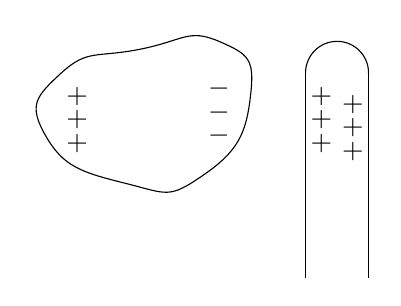
\begin{tikzpicture}

  % Shape of the object
  \path[draw=black]
    plot[smooth cycle, tension=1] coordinates {
      (0,0.4) (1,0.5) (1.4,-0.2)
      (0.8,-1.2) (-0.2,-1.3)
      (-1.2,-0.7) (-1,0.1)
    };

	\node at (-0.8,-0.2) {$+$};
	\node at (-0.8,-0.5) {$+$};
	\node at (-0.8,-0.8) {$+$};

	\node at (1.0,-0.1) {$-$};
	\node at (1.0,-0.4) {$-$};
	\node at (1.0,-0.7) {$-$};


	\draw (2.1,0.1) -- (2.1,-2.5);
	\draw (2.9,0.1) -- (2.9,-2.5);
	\draw (2.1,0.1) arc[start angle=180, end angle=0, radius=4mm];

	\node at (2.3,-0.2) {$+$};
	\node at (2.3,-0.5) {$+$};
	\node at (2.3,-0.8) {$+$};

	\node at (2.7,-0.3) {$+$};
	\node at (2.7,-0.6) {$+$};
	\node at (2.7,-0.9) {$+$};

\end{tikzpicture}
  \caption{Positively charged rod next to some conductive object}
  \label{fig:charged-rod}
\end{figure}

What happens in Figure~\ref{fig:charged-rod} mostly due to induction where the atoms become polarized, i.e., the electron spends more time on one side than the other.
\begin{figure}[H]
\centering
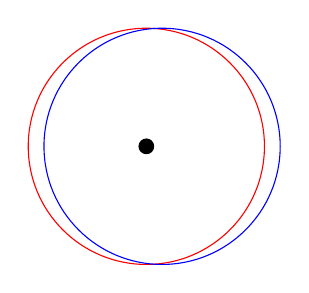
\begin{tikzpicture}

  \fill (0,0) circle (1mm);
  \draw[red] (0,0) circle (15mm);
  \draw[blue] (0.2,0) circle (15mm);

	\end{tikzpicture}
  \caption{Polarized atom is shown with the blue circle and red is non polarized.}
  \label{fig:polarized-atom}
\end{figure}

\begin{figure}[H]
     \centering
     \begin{subfigure}[b]{0.4\textwidth}
         \centering
         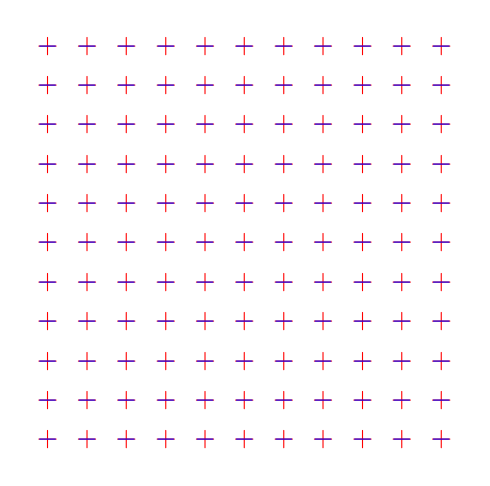
\begin{tikzpicture}

          \foreach \y in {0,1,...,10}
          {
            \foreach \x in {0,1,...,10}
            {
              \pgfmathtruncatemacro{\xnegpos}{0.5*\x + 0.02};
              \pgfmathtruncatemacro{\ynegpos}{0.5*\y + 0.02};
              \node[red] at (0.5*\x,0.5*\y) {$+$};
              \node[blue] at (0.5*\x,0.5*\y) {$-$};
            }
          }

         \end{tikzpicture}
         \caption{No induction, where $-$ is over $+$.}
         \label{fig:y equals x}
     \end{subfigure}
     \hfill
     \begin{subfigure}[b]{0.4\textwidth}
         \centering
          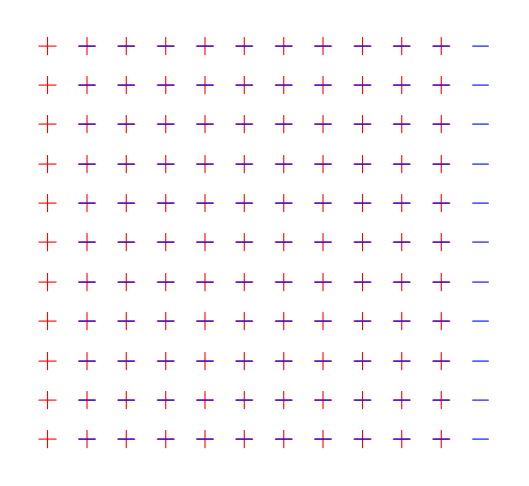
\begin{tikzpicture}


          \foreach \y in {0,...,10}
          {
            \foreach \x in {0,...,10}
            {
              \node[red] at (0.5*\x,0.5*\y) {$+$};
            }
            \foreach \x in {1,...,11}
            {
              \node[blue] at (0.5*\x,0.5*\y) {$-$};
            }
          }


         \end{tikzpicture}
         \caption{Induction, where $-$ is shifted to the right.}
         \label{fig:three sin x}
     \end{subfigure}
        \caption{No induction compared to induction.}
        \label{fig:three graphs}
\end{figure}

\section{Electric Forces and Coulomb's Law}
%31:50 Coulomb's Law 
%40:00 what holds the world together, the autom scale the neculer force, then the electric force and on the size of planets and galixies it is the gravitational force. why
Coulomb's law describes the force resulted by two charged points $q_1$ and $q_2$, separated by a distance $r$ in vacuum.
\begin{equation}
  \vec{\boldsymbol{F}}_{12} = k_e \frac{q_1q_2}{r^2}\hat{\boldsymbol{r}}
\end{equation}
where $k_e$ is Coulomb's constant. $\hat{\boldsymbol{r}}$ is the unit vector directed from $q_1$ and $q_2$ defined as $\hat{\boldsymbol{r}}=\vec{\boldsymbol{r}}/r$.
See Figure~\ref{fig:coulomb-illustration} for the illustration of Coulomb's law.

\begin{figure}[H]
\centering
     \centering
     \begin{subfigure}[b]{0.45\textwidth}
         \centering
  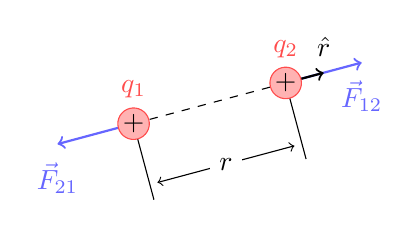
\begin{tikzpicture}

	\begin{scope}[rotate=15] 
    \draw[thick, blue!60, ->] (0,0) -- (-1,0) node[below=1mm] {$\vec{\boldsymbol{F}}_{21}$};  
    \draw[thick, blue!60, ->] (2,0) -- (3,0) node[below=1mm] {$\vec{\boldsymbol{F}}_{12}$}; 
    \draw[thick, ->] (2,0) -- (2.5,0) node[above=0.8mm] {$\hat{\boldsymbol{r}}$}; 

    \draw[dashed] (0,0) -- (2,0); 
    \draw (0,0) -- (0,-1);
    \draw (2,0) -- (2,-1);
    \draw[<->](0.1,-0.8)--(1.9,-0.8) node[midway,fill=white]{$r$};

    \filldraw[color=red!70, fill=red!30] (0,0) circle (2mm) node[above=2mm] {$q_1$};
    \node at (0,0) {$+$}; 
    \filldraw[color=red!70, fill=red!30] (2,0) circle (2mm) node[above=2mm] {$q_2$};
    \node at (2,0) {$+$}; 
  \end{scope}

	\end{tikzpicture}
  \caption{Repel.}
  \label{fig:coulomb-illustration-repel}
  \end{subfigure}
     \hfill
  \begin{subfigure}[b]{0.45\textwidth}
    \centering
  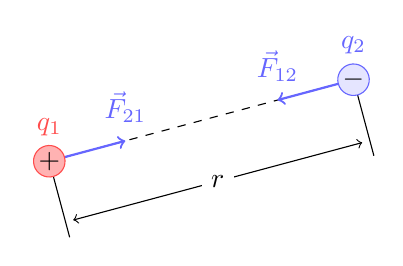
\begin{tikzpicture}

	\begin{scope}[rotate=15] 
    \draw[dashed] (0,0) -- (4,0); 
    \draw (0,0) -- (0,-1);
    \draw (4,0) -- (4,-1);
    \draw[<->](0.1,-0.8)--(3.9,-0.8) node[midway,fill=white]{$r$};

    \draw[thick, blue!60, ->] (0,0) -- (1,0) node[above=1mm] {$\vec{\boldsymbol{F}}_{21}$};  
    \draw[thick, blue!60, ->] (4,0) -- (3,0) node[above=1mm] {$\vec{\boldsymbol{F}}_{12}$}; 


    \filldraw[color=red!70, fill=red!30] (0,0) circle (2mm) node[above=2mm] {$q_1$};
    \node at (0,0) {$+$}; 
    \filldraw[color=blue!60, fill=blue!10] (4,0) circle (2mm) node[above=2mm] {$q_2$};
    \node at (4,0) {$-$}; 
  \end{scope}

	\end{tikzpicture}
  \caption{Attracted.}
  \label{fig:coulomb-illustration-attracted}
  \end{subfigure}

  \caption{Illustration of Coulomb's Law.}
  \label{fig:coulomb-illustration}
\end{figure}

Coulomb's constant $k_e$ is defined as:
\begin{equation*}
  k_e = \frac{1}{4\pi\varepsilon_0} = \SI[per-mode = fraction]{8.9875e9}{\newton\meter\squared\per\coulomb\squared}
\end{equation*}
where $\varepsilon_0$ is the \textbf{Vacuum Permittivity}, also known as the
\textbf{Electric Constant} or the \textbf{Permittivity of Free Space}, i.e., a
measure of how much resistance the vacuum of empty space puts up against an
electric field.
\begin{equation*}
  \varepsilon_0 = \SI[per-mode = fraction]{8.85e-12}{\coulomb\squared\per\newton\meter\squared}
\end{equation*}


\section{Principle of Superposition}
Coulomb's laws applies to a pair of charged points and when there are more than
two charged points the net force on any charged point is the vector sum of all
forces exerted on it by the other changed points. 
\begin{equation*}
  \vec{\boldsymbol{F}}_{j} = \sum_{\substack{i=1 \\ j \neq i}}^{N} \vec{\boldsymbol{F}}_{ij}
\end{equation*}
where $\vec{\boldsymbol{F}}_{ij}$ denotes the force between charged point $i$ and $j$ for a system of $N$ charges.

\paragraph{Example:}
There are three charged points shown in Figure~\ref{fig:system-of-three-charges}. Find the force on charge $q_3$, when $q_1 = \SI{6.0e-6}{\coulomb}$, $q_2 = -q_1 = \SI{-6.0e-6}{\coulomb}$, $q_3 = \SI{3.0e-6}{\coulomb}$, and $\SI{2.0e-2}{\meter}$.

\begin{figure}[H]
\centering
\begin{tikzpicture}

  \draw (0,0) -- (0,4) node[above] {$y$} node[pos=0.4, left] {$a$};
  \draw (0,0) -- (4,0) node[right] {$x$};
  \draw[dashed] (0,0) -- (3,3) node[midway, below] {$\sqrt{2}a$};
  \draw[dashed] (3,3) -- (5,3);
  \draw (0,3) -- (3,3);
  \draw[dashed] (0.5,3) -- (1.5,4);
  \draw[dashed] (1.5,4) -- (4,4);
  \draw[thick] (1,0) arc[start angle=0, end angle=45, radius=10mm] node[midway, right] {$\theta$};
  \draw[thick, dashed, -Stealth] (4.5,3) arc[start angle=45, end angle=110, radius=20mm] node[midway, right=3mm] {$\phi$};

  \draw[color=blue!60, very thick, -Stealth] (3,3) -- (0.5,3) node[below] {$\vec{\boldsymbol{F}}_{23}$};
  \draw[color=blue!60, very thick, -Stealth] (3,3) -- (1.5,4) node[above] {$\vec{\boldsymbol{F}}_{3}$};
  \draw[color=blue!60, very thick, -Stealth] (3,3) -- (4,4) node[above right] {$\vec{\boldsymbol{F}}_{13}$};

  \draw[very thick, -Stealth] (3,3) -- (3.5,3.5) node[below right=0.5mm] {$\hat{\boldsymbol{r}}_{13}$};;
  \draw[very thick, -Stealth] (3,3) -- (3.8,3) node[below] {$\hat{\boldsymbol{r}}_{23}$};

  \filldraw[color=red!70, fill=red!30] (0,0) circle (2mm) node[left=2mm] {$q_1$};
  \node at (0,0) {$+$}; 
  \filldraw[color=blue!60, fill=blue!10] (0,3) circle (2mm) node[left=2mm] {$q_2$};
  \node at (0,3) {$-$}; 
  \filldraw[color=red!70, fill=red!30] (3,3) circle (2mm) node[below=2mm] {$q_3$};
  \node at (3,3) {$+$}; 

\end{tikzpicture}
  \caption{A system of three charges.}
  \label{fig:system-of-three-charges}
\end{figure}


\subparagraph{Solution:}
Using the super position principle, the force on $q_3$ is
\begin{equation*}
  \vec{\boldsymbol{F}}_{3} = \vec{\boldsymbol{F}}_{13} +
  \vec{\boldsymbol{F}}_{23} = \frac{1}{4\pi\varepsilon_0} \left(
  \frac{q_1q_3}{r^2_{13}}\hat{\boldsymbol{r}}_{13} + \frac{q_2q_3}{r^2_{23}}\hat{\boldsymbol{r}}_{23} \right)
\end{equation*}
where the unit vector $\hat{\boldsymbol{r}}_{13}$ is 
\begin{equation*}
  \hat{\boldsymbol{r}}_{13} = \cos{\theta}\hat{\boldsymbol{i}} + \cos{\theta}\hat{\boldsymbol{j}} = \frac{\sqrt{2}}{2}(\hat{\boldsymbol{i}} + \hat{\boldsymbol{j}})
\end{equation*}
and $\hat{\boldsymbol{r}}_{23} = \hat{\boldsymbol{i}}$. Therefore, the total force is 
\begin{align*}
  \vec{\boldsymbol{F}}_{3} &= \frac{1}{4\pi\varepsilon_0} \left(
  \frac{q_1q_3}{r^2_{13}}\hat{\boldsymbol{r}}_{13} + \frac{q_2q_3}{r^2_{23}}\hat{\boldsymbol{r}}_{23} \right)
  = \frac{1}{4\pi\varepsilon_0} \left(
  \frac{q_1q_3}{(\sqrt{2}a)^2}\frac{\sqrt{2}}{2}(\hat{\boldsymbol{i}} + \hat{\boldsymbol{j}}) 
  + \frac{(-q_1)q_3}{a^2}\hat{\boldsymbol{i}} \right) \\
  &= \frac{1}{4\pi\varepsilon_0} \frac{q_1q_3}{a^2} \left(\left(
  \frac{\sqrt{2}}{4}-1\right)\hat{\boldsymbol{i}} + \frac{\sqrt{2}}{4}\hat{\boldsymbol{j}} \right) 
\end{align*}
The total force, i.e., the ``length'' of the vector, can be calculated by pythagorean theorem $c=\sqrt{a^2+b^2}$, which gives us
\begin{align*}
  \vec{\boldsymbol{F}}_{3} 
  &= \frac{1}{4\pi\varepsilon_0} \frac{q_1q_3}{a^2} \sqrt{\left(
  \frac{\sqrt{2}}{4}-1\right)^2 + \left(\frac{\sqrt{2}}{4}\right)^2 } \\
  &= \left(\SI[per-mode =
  fraction]{9.0e9}{\coulomb\squared\per\newton\meter\squared}\right)
  \frac{(\SI{6.0e-6}{\coulomb})(\SI{3.0e-6}{\coulomb})}{(\SI{2.0e-2}{\meter})^2}
  (0.74) = \SI{3.0}{\newton}
\end{align*}
The angle of the force from the x-axis is
\begin{equation*}
  \phi = \arctan{\left( \frac{F_{3,y}}{F_{3,x}} \right)}
  = \arctan{\left( \frac{\sqrt{2}/4}{-1+\sqrt{2}/4} \right)} = \SI{151.3}{\degree}
\end{equation*}



\section{Electric Fields}
%Force fields, shows the vectors of attraction and repelence due to electrical charges
%7:00 Sum of the individual elements of the charges
%Are also field lines not just a vector field
%25:55 Whould be in to have a field shouwing an atom that the electrons want to spend more time on one side than the other
%Dipole

\begin{figure}[H]
\centering
  \begin{subfigure}[b]{0.45\textwidth}
    \centering
\begin{tikzpicture}[
    scale=0.80,
    attach arrow/.style args={#1}{
        decoration={
            markings,
            mark=at position 0 with {\pgfextra{%
                \pgfmathsetmacro{\tmpArrowTime}{\pgfkeysvalueof{/tikz/arc arrow/length}/(\pgfdecoratedpathlength)}%
                \xdef\tmpArrowTime{\tmpArrowTime}}},
            mark=at position {#1-3*\tmpArrowTime} with {\coordinate(@1);},
            mark=at position {#1-2*\tmpArrowTime} with {\coordinate(@2);},
            mark=at position {#1-1*\tmpArrowTime} with {\coordinate(@3);},
            mark=at position {#1+\tmpArrowTime/2} with {\coordinate(@4);
                \draw[-{Stealth[length=\pgfkeysvalueof{/tikz/arc arrow/length},bend]}]
                  plot[smooth] coordinates {(@1) (@2) (@3) (@4)};},
        },
        postaction=decorate,
    },
    attach arrow/.default=0.5,
    arc arrow/.cd, length/.initial=2mm,
]
\node[draw=red!70, fill=red!30, circle, minimum size=6mm] (Q) {+};

% Radial outward field lines
\foreach \a in {0,30,...,330} {
  \draw[red!70, thick, attach arrow={1/3}, attach arrow={2/3}] (Q) -- ++(\a:3);
}
\end{tikzpicture}
  \caption{}
  \label{fig:electric-field-line-for-positive}
  \end{subfigure}
     \hfill
  \begin{subfigure}[b]{0.45\textwidth}
    \centering
\begin{tikzpicture}[
    scale=0.80,
    attach arrow/.style args={#1}{
        decoration={
            markings,
            mark=at position 0 with {\pgfextra{%
                \pgfmathsetmacro{\tmpArrowTime}{\pgfkeysvalueof{/tikz/arc arrow/length}/(\pgfdecoratedpathlength)}%
                \xdef\tmpArrowTime{\tmpArrowTime}}},
            mark=at position {#1-3*\tmpArrowTime} with {\coordinate(@1);},
            mark=at position {#1-2*\tmpArrowTime} with {\coordinate(@2);},
            mark=at position {#1-1*\tmpArrowTime} with {\coordinate(@3);},
            mark=at position {#1+\tmpArrowTime/2} with {\coordinate(@4);
                \draw[-{Stealth[length=\pgfkeysvalueof{/tikz/arc arrow/length},bend]}]
                  plot[smooth] coordinates {(@1) (@2) (@3) (@4)};},
        },
        postaction=decorate,
    },
    attach arrow/.default=0.5,
    arc arrow/.cd, length/.initial=2mm,
]
\node[draw=blue!70, fill=blue!20, circle, minimum size=6mm] (Q) {$-$};

% Radial inward field lines
\foreach \a in {0,30,...,330} {
  \draw[red!70, thick, attach arrow={1/3}, attach arrow={2/3}] ++(\a:3) -- (Q);
}
\end{tikzpicture}
  \caption{}
  \label{fig:electric-field-line-negative}
  \end{subfigure}
  \caption{Field lines for (a) positive, radially outwards, and (b) negative charges, radially inwards.}
  \label{fig:electric-field-lines}
\end{figure}


\begin{figure}[H]
\centering
\begin{tikzpicture}[
    scale=1,
    attach arrow/.style={
        decoration={
            markings,
            mark=at position 0 with {\pgfextra{%
                \pgfmathsetmacro{\tmpArrowTime}{\pgfkeysvalueof{/tikz/arc arrow/length}/(\pgfdecoratedpathlength)}%
                \xdef\tmpArrowTime{\tmpArrowTime}}},
            mark=at position {#1-3*\tmpArrowTime} with {\coordinate(@1);},
            mark=at position {#1-2*\tmpArrowTime} with {\coordinate(@2);},
            mark=at position {#1-1*\tmpArrowTime} with {\coordinate(@3);},
            mark=at position {#1+\tmpArrowTime/2} with {\coordinate(@4);
                \draw[-{Stealth[length=\pgfkeysvalueof{/tikz/arc arrow/length},bend]}] plot[smooth]
                coordinates {(@1) (@2) (@3) (@4)};},
        },
        postaction=decorate,
    },
    attach arrow/.default=0.5,
    arc arrow/.cd,length/.initial=2mm,
    %nodes={circle,minimum size=2.4em,font=\bfseries\sffamily}
]
\path 
    node[draw=red!70, fill=red!30, circle, minimum size=6mm] (L){+} 
    (2.5,0) node[draw=blue!60, fill=blue!10, circle, minimum size=6mm] (R){--};
\foreach \X in {0,...,7}
 {\draw[red!70, thick, attach arrow] (L) 
 to[bend left={-70+\X*20},looseness=1.6] 
 (R);}
\foreach \X in {0,...,10}
 {\draw[red!70, thick,attach arrow/.list={1/3,2/3}] (L) to[bend left=16-4*\X] ++ (70+\X*22:3);
 \draw[red!70, thick,attach arrow/.list={1/3,2/3}] (R)+(180+70+\X*22:3) 
 to[bend right=16-4*\X] 
  (R);}
\end{tikzpicture}
  \caption{Field lines for an electric dipole.}
  \label{fig:electric-field-line-for-dipole}
\end{figure}



%\section{Coulomb's Law}
\section{Electric Potential}
\section{Gauss' Law}
\section{Capacitors}
\section{Current and Resistance}
\section{Direct Current Circuits}
\section{Magnetic Fields}
\section{Sources of Magnetic Fields}
\section{Faraday's Law}
\section{Inductance and Energy in Magnetic Fields}
\section{Alternating Current Circuits}
\section{Maxwell's Equations and Electromagnetic Waves}
\section{Interference and Diffraction}


